%% Submissions for peer-review must enable line-numbering
%% using the lineno option in the \documentclass command.
%%
%% Preprints and camera-ready submissions do not need
%% line numbers, and should have this option removed.
%%
%% Please note that the line numbering option requires
%% version 1.1 or newer of the wlpeerj.cls file, and
%% the corresponding author info requires v1.2

\documentclass[fleqn,10pt]{wlpeerj} % for preprint submissions

% ZNK -- Adding headers for pandoc

\setlength{\emergencystretch}{3em}
\providecommand{\tightlist}{
\setlength{\itemsep}{0pt}\setlength{\parskip}{0pt}}
\usepackage{lipsum}
\usepackage[unicode=true]{hyperref}
\usepackage{longtable}



\usepackage{lipsum} \usepackage{float}

\title{Juvenile Salmon Migration Observations in the Discovery Islands and Johnstone Strait in 2018}

\author[1]{Brett T. Johnson}

\corrauthor[1]{Brett T. Johnson}{\href{mailto:brett.johnson@hakai.org}{\nolinkurl{brett.johnson@hakai.org}}}
\author[]{Julian C.L. Gan}

\author[]{Carly V. Janusson}

\author[1, 2, 3]{Brian P.V. Hunt}


\affil[1]{Hakai Institute Quadra Island Ecological Observatory, Heriot Bay, BC V0P 1H0}
\affil[2]{Institute for the Oceans and Fisheries, University of British Columbia Vancouver, B.C., Canada V6T 1Z4}
\affil[3]{Department of Earth, Ocean and Atmospheric Sciences, University of British Columbia Vancouver, B.C., Canada V6T 1Z4}


%
% \author[1]{First Author}
% \author[2]{Second Author}
% \affil[1]{Address of first author}
% \affil[2]{Address of second author}
% \corrauthor[1]{First Author}{f.author@email.com}

% 

\begin{abstract}
Out-migrating juvenile Fraser River sockeye (\emph{Oncorhynchus} \emph{nerka}), pink (\emph{O.} \emph{gorbuscha}), and chum (\emph{O.} \emph{keta}) salmon pass northwest through the Strait of Georgia, the Discovery Islands, and Johnstone Strait---a region of poor survival for juvenile salmon relative to the Strait of Georgia. To better understand the factors that drive early marine survival through this region, the Hakai Institute Juvenile Salmon Program monitors critical aspects of this migration by capturing migrating salmon between May and July each year using a purse seine. Here we report on the 2018 observations in comparison to averages from our 2015--2018 time series. In 2018 sockeye, pink, and chum migration timing was not significantly different than time series averages. The median capture date across years in the Discovery Islands was May 23 for sockeye and June 12 for pink and chum. Pink salmon comprised the highest proportion of the catch and the highest average catch intensity in 2018, followed by chum and then sockeye. Sockeye were longer than average in 2018, whereas pink and chum were smaller than average (all \emph{p} \textless{} 0.001). In the Discovery Islands, sea-louse abundance in 2018 was lower than average for sockeye, pink, and chum. In Johnstone Strait, sea-louse abundance was lower for chum but higher than average for sockeye and pink. Notably, there were no \emph{Lepeophtheirus salmonis} sea lice observed in Johnstone Strait in 2018. Sea-surface temperatures in the northern Strait of Georgia during the smolt migration period of 2018 were the warmest on record in the study period.
% Dummy abstract text. Dummy abstract text. Dummy abstract text. Dummy abstract text. Dummy abstract text. Dummy abstract text. Dummy abstract text. Dummy abstract text. Dummy abstract text. Dummy abstract text. Dummy abstract text.
\end{abstract}

\begin{document}

\flushbottom
\maketitle
\thispagestyle{empty}

\hypertarget{introduction}{%
\section{Introduction}\label{introduction}}

The first months after marine entry have been identified as a potentially critical period for salmon stock recruitment (Beamish and Mahnken 2001), which may ultimately be responsible for inter-annual variability and long-term declines in British Columbian salmon stocks (Peterman et al. 2010; Beamish et al. 2012). Pathogens, parasites, predators, and the impacts of climate change on food web dynamics have emerged as leading causes for the declines (\#TODO: add reference). The Hakai Institute Juvenile Salmon Program has been monitoring juvenile salmon migrations in the Discovery Islands and Johnstone Strait (Figure \ref{fig:map}) since 2015 in an effort to understand the factors that are influencing early marine survival of sockeye, pink, and chum (Hunt et al. 2018). This report summarizes migration timing, fish length, parasite loads, species composition, and sea-surface temperature observed from the first 4 years of this research and monitoring program. These estimates will provide context to investigate questions and interpret results related to growth, survival, and the conditions salmon experience during their migration through this critical region.

\begin{figure}[H]

\includegraphics[width=0.9\linewidth]{map} \hfill{}

\caption{Sampling locations in 2018}\label{fig:map}
\end{figure}

\hypertarget{methods}{%
\section{Methods}\label{methods}}

\hypertarget{field-methods}{%
\subsection{Field methods}\label{field-methods}}

See Hunt et al. (2018) for a detailed description of field and lab methods. Briefly, juvenile salmon were collected weekly from the Discovery Islands and Johnstone Strait during their northward migration from the Strait of Georgia to Queen Charlotte Strait near northern Vancouver Island, British Columbia. We sampled from May to July each year, beginning in 2015, using hand-operated purse seine nets (bunt: 27 m x 9 m with 13 mm mesh; tow: 46 m x 9 m with 76 mm mesh) (Godwin et al. 2015). We sampled near-shore marine habitats where depth was \textgreater{} 10 m, effectively sampling sockeye (\emph{Oncorhynchus nerka}), pink (\emph{O. gorbuscha}) and chum (\emph{O. keta}) salmon, and incidentally captured coho (\emph{O. kisutch}), Chinook (\emph{O. tshawytschya}) and Pacific herring (\emph{Clupea pallasii}). All animal care was in accordance with Animal Care Guidelines under permit A16-0101. We collected temperature data by deploying an RBR conductivity, temperature, and depth profiler to depths \textgreater{} 30 m at station QU39 (Figure \ref{fig:map}) in the northern Strait of Georgia.

\hypertarget{data-analysis}{%
\subsection{Data Analysis}\label{data-analysis}}

Time series anomalies reported are in relation to the time series averages (2015-2018). Measurements from the Discovery Islands and Johnstone Strait regions of the salmon migration were combined in analyses unless otherwise indicated. Only sites that were sampled in all years were used. All analyses were conducted using R (R Core Team 2017).

Add clarifying sentence here about why abundance and catch intensity is based on seines that contained sockeye.

The peak migration date for each species was estimated by calculating the median date of capture in the Discovery Islands. This method was used because the period in which surveys and seines were conducted was the same each year and seines were always conducted before sockeye arrived and after sockeye disappeared. Often, however, the entire duration of the pink and chum migration through the Discovery Islands was not captured because their migration period is more protracted compared to sockeye. Cumulative abundance was calculated over a constrained period between May 1 and July 9 of each year to standardize the period over which cumulative abundance was calculated. Because the Fraser River is currently an even-year-dominant system for pink salmon, very few out-migrating pink are caught in odd years; consequently, only even years were included in the calculation of the pink time series average.

In 2015 and 2016 we focussed on capturing sockeye and we only enumerated and sampled other species such as pink and chum when sockeye were caught. As a result, catch statistics such as catch intensity and proportion reflect the fact that we only unumerated and sampled salmon when sockeye were caught. In 2017 and 2018 all seines that captured any species of salmon were enumerated and sampled. These differences in methodology are reflected in the way catch intensity and catch proportions are calculated in so far as catch intensity and catch proportion calculations are restricted to when sockeye were present.

Catch intensity was calculated to provide a measure of inter-annual abundance for sockeye, pink, and chum. Catch intensity was defined as the average number of a species caught when \textgreater{} 1 of that particular species was caught, and when sockeye were also caught. In effect, catch intensity summarizes the abundance of each species in a community of co-migrating sockeye, pink, and chum when sockeye are present.

Species proportions were calculated by dividing the total number of each species caught by the sum of all species caught that season. Only seines that caught sockeye were used in the calculation of species to represent the salmon community composition that co-migrate with sockeye. To test whether fork lengths from 2018 were significantly different than the time series averages, an independent two-group t-test was conducted. Fork length distributions were visualized by calculating length frequency distributions using kernel density estimates from fork length data.

The prevalence, intensity, and abundance of \emph{Caligus clemensi} and \emph{Lepeophtheirus salmonis} sea lice were calculated according to the definitions in Margolis et al. (1990). Only motile (i.e., pre-adult and adult) stages were included in analyses while nauplius, copepodid, and chalimus life stages were excluded.

The mean sea-surface temperature (SST) was calculated from the top 30 m of the water column in May and June--the period during which salmon migrate through the region. To visualize temperature anomalies, a LOESS regression was applied to sea-surface temperatures from all years to represent the average seasonal trend.

\hypertarget{results-and-discussion}{%
\section{Results and Discussion}\label{results-and-discussion}}

Most migration parameters were below average in 2018 except for sockeye length and SST (Figure \ref{fig:heatmap}). Interestingly, sockeye length tends to be the opposite anomaly compared to pink and chum which vary together.

Migration timing in the Discovery Islands in 2018 did not differ from the time series average by more than a week for sockeye, pink, or chum (Figure \ref{fig:migration-timing-plot}) (Table \ref{tab:migration-timing-table}). The peak migration date for sockeye in the Discovery Islands was on May 23, 5 days earlier than the time series average of May 28. The peak migration date for pink in the Discovery Islands was on June 12, 1 days earlier than the average of June 13. The peak migration date for chum in the Discovery Islands was on June 12, 3 days earlier than the average of June 15. The expected accuracy of these estimates is +/- 5-7 days.

Sockeye run timing is highly left-skewed and the number of days between the 25th and 50th percentile of catch abundnance was 2 days on average, indicating that there is a puncuated event that illicits their northerly migration (Table \ref{tab:migration-timing-table}). In 2014, a DFO purse seiner measured 80\% of sockeye passing through the Discovery Islands between June 12 and June 19th (Neville et al. 2016). The interquartile range for sockeye migration timing we averaged for 2015--2018 is May 26--June 4, roughly two and a half weeks earlier than observed in 2014. Sockeye from 2014 and 2017 are from the same cyclic dominance cohort. The year 2017 exhibited the latest migration timing of all four run cycles, suggesting that this run cycle tends to migrate later than the others. Sockeye leave the Strait of Georgia 12-20 days before pink and chum. This is driven mostly by water temperatures (REF), in addition to better foraging conditions on the continental shelf where upwelling nutrients contribute to higher productivity (Ref). However, sea-surface temperatures in the northern Strait of Georgia in 2017 were the coolest between 2015--2017, confounding the interpretation of the late 2014/2017 run cycle if you assume that sea-surface temperature is what predominantly drives juvenile salmon to migrate north of the Strait of Georgia.

In 2017 Chum migrations were also later than average, and as a result the tail end of the migration was not completely captured. In 1983, two trawl surveys were conducted in Discovery Passage and the surrounding channels and found that pink and chum abundance peaked in late June.

Sockeye catch intensity in 2018 was low relative to sockeye in previous years and relative to pink and chum in 2018 (Figure \ref{fig:catch-intensity-plot}). That sockeye catch intensity was low in 2018 is not surprising because 2016 brood year Shuswap or Chilko Lake sockeye, two stocks which are among the most productive, are not as abundant in this cohort as they are in others. Pink catch intensity in 2018 was the highest of the four years measured. Pink out-migrants are more abundant on even years, the result of the odd-year dominant life-cycle of Fraser River pinks (Heard 1991), but 2018 catches indicate either good production or good survival in the early marine environment for pink salmon relative to 2016---the only other odd-year dominant brood year recorded by the Juvenile Salmon Program.

Pink salmon dominated the catch in the Discovery Islands and Johnstone in 2018 making up 51.5 \% of the catch (Table \ref{tab:proportion-table}) while chum made up 32.6 \% and sockeye 13.1 \% (Figure \ref{fig:proportion-plot}). This was the first time in the time series that pink dominated the catch proportion.

Fish lengths varied between regions, and among species and years (Figure \ref{fig:length-plot}) though in 2018 sockeye were longer, pink were shorter, and chum were shorter than their respective time series averages in the Discovery Islands and Johnstone Strait combined. Sockeye length was 116.9 mm (Table \ref{tab:length-table}), which is 8.3 mm longer than the time series average (\emph{p} \textless{} 0.0001, 95\% CI 5.5 -11.2). Average pink lengths were 96.4 mm, which is 9.5 mm shorter than the time series average (\emph{p} \textless{} 0.0001, 95\% CI 11.8-7.2). Chum were on average 103.5 mm, which is 7.9 mm shorter than the time series average (\emph{p} \textless{} 0.0001, 95\% CI 9.9--5.8).

The abundance of motile sea lice in 2018 was the among the lowest recorded in the Discovery Islands time-series while Johnstone Strait parasite loads were average. (Figure \ref{fig:sealice-abundance-plot}). Notably, no \emph{Lepeophtheirus salmonis} were detected on sockeye in Johnstone Strait, despite being present in the Discovery Islands. The time series averages indicate pink salmon have higher sea lice abundance, prevalence, and intensity compared to the chum, and sockeye (Table \ref{tab:sealice-table}) in contrast to Patanasatienkul et al. (2013) where they found that the prevalence and intensity of sea lice was higher on chum than pink on early marine entrants in the Broughton Archipelago.

Sea-surface temperature in May and June during the juvenile salmon out-migration at QU39 in the northern Strait of Georgia was 0.28 degrees C warmer than average (Table \ref{tab:sst-table}) (Figure \ref{fig:sst-plot}). In the context of the last four last years 2018 was the warmest surface waters observed in the northern Strait of Georgia, despite 2015 SST along the BC coast breaking records for high temperatures (Chandler, King, and Boldt 2017).

\begin{figure}[H]
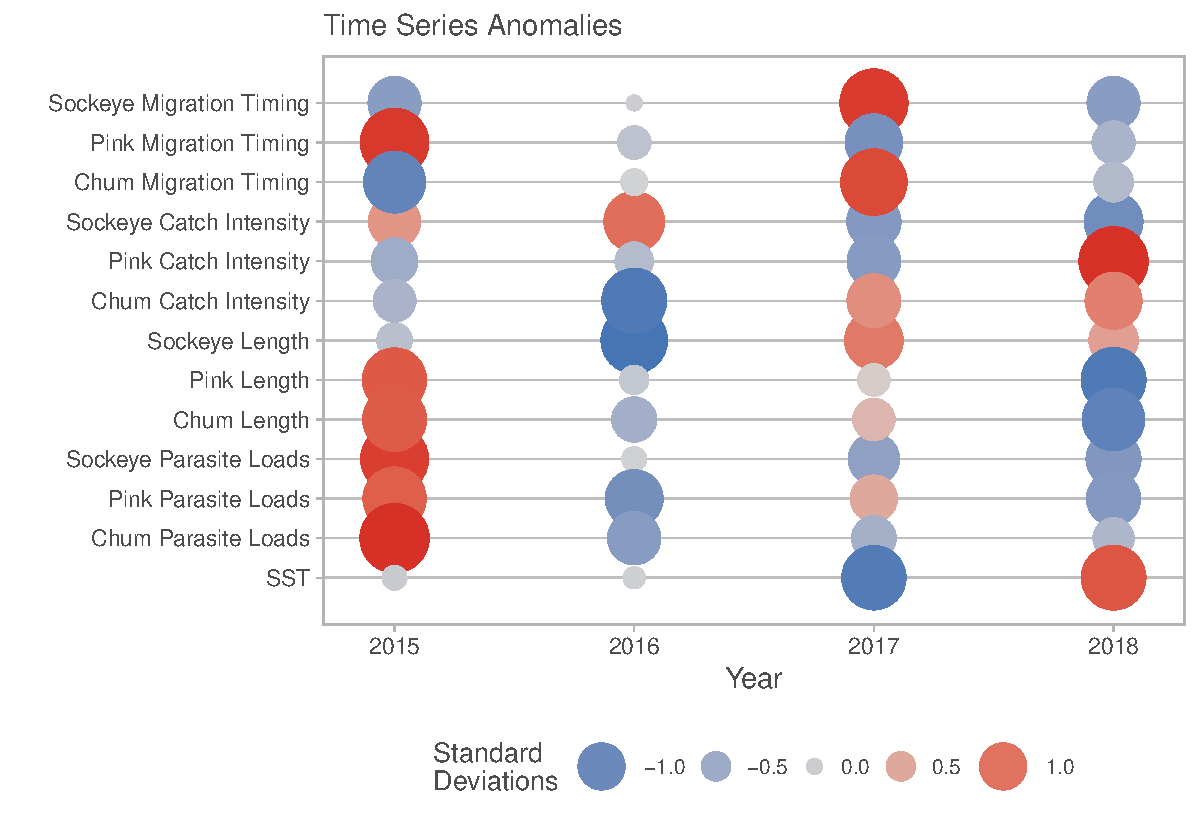
\includegraphics[width=0.95\linewidth]{Migration_Observations_Report_files/figure-latex/heatmap-1} \caption{This heatmap indicates the number of standard deviations (z-score) from the time series average (2015-2018) for key migration parameters. Size and colour saturation of circles indicates magnitude of the anomaly. Blue colour indicates less than average, grey indicates average, red indicates greater than average. Peak migration date is based on the median date of fish capture in the Discovery Islands. Length is based on the average fork length from the Discovery Islands and Johnstone Strait combined. Parasite load is the average abundance of all sea-louse species in their motile life stages for both the Discovery Islands and Johnstone Strait regions. “SST” describes the mean sea-surface temperature in the top 30 m at station QU39 in the northern Strait of Georgia in May and June.}\label{fig:heatmap}
\end{figure}

\begin{figure}[H]
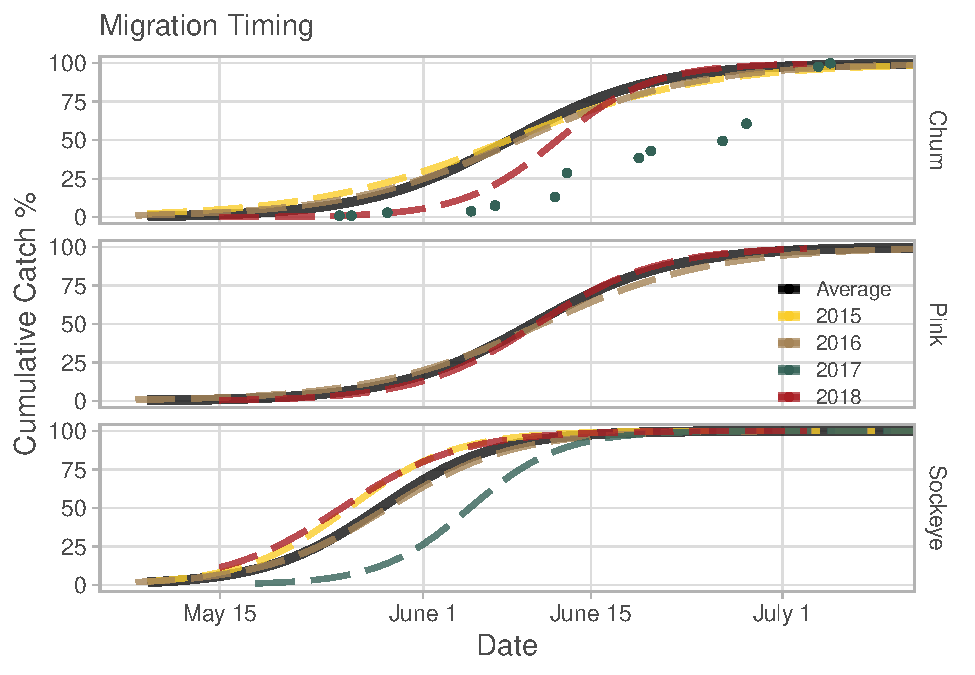
\includegraphics[width=0.9\linewidth]{Migration_Observations_Report_files/figure-latex/migration-timing-plot-1} \caption{Cumulative annual abundance of sockeye, pink, and chum, in the Discovery Islands and Johnstone Strait compared to the time series average.}\label{fig:migration-timing-plot}
\end{figure}

\begin{figure}
\centering
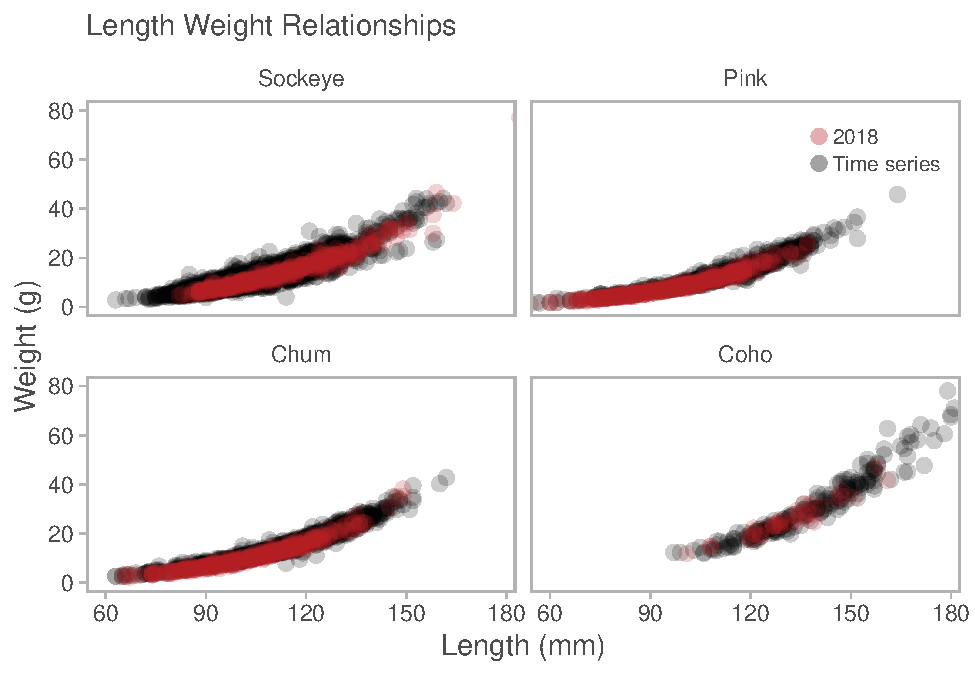
\includegraphics{Migration_Observations_Report_files/figure-latex/condition-plot-1.pdf}
\caption{\label{fig:condition-plot}Length and weight regressions for juvenile salmon caught in the Discovery Islands and Johnstone Strait in 2018 coloured red, compared to all outher years in black.}
\end{figure}

\begin{figure}[H]
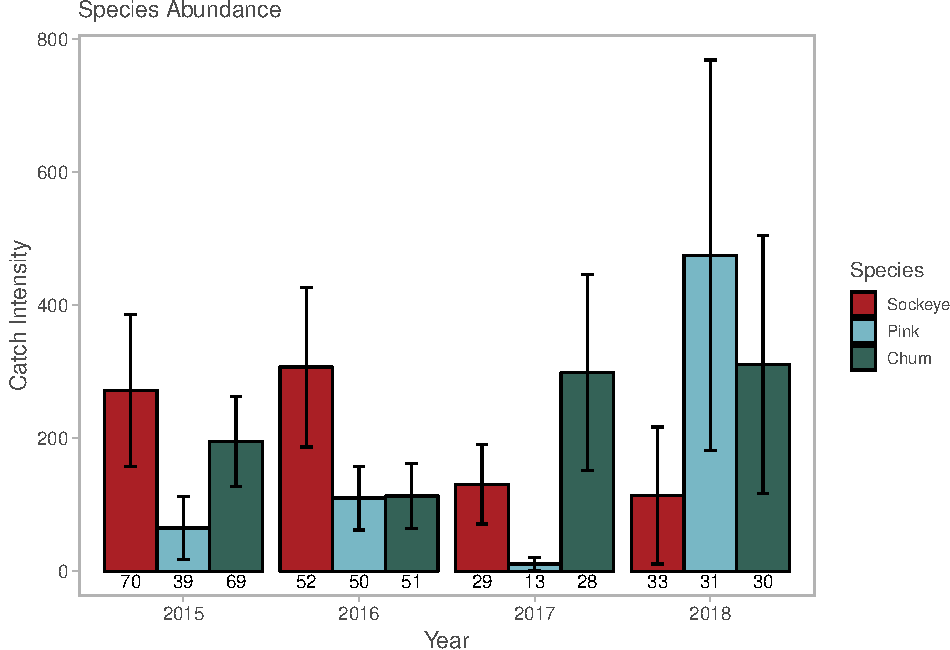
\includegraphics[width=0.9\linewidth]{Migration_Observations_Report_files/figure-latex/catch-intensity-plot-1} \caption{The catch intensity (our proxy for abundance) of sockeye, pink, and chum salmon in the Discovery Islands and Johnstone Strait. Numbers under each bar indicate the number of seines in which the species was caught, and erorr bars indicate the 95 percent confidence region.}\label{fig:catch-intensity-plot}
\end{figure}

\begin{figure}[H]
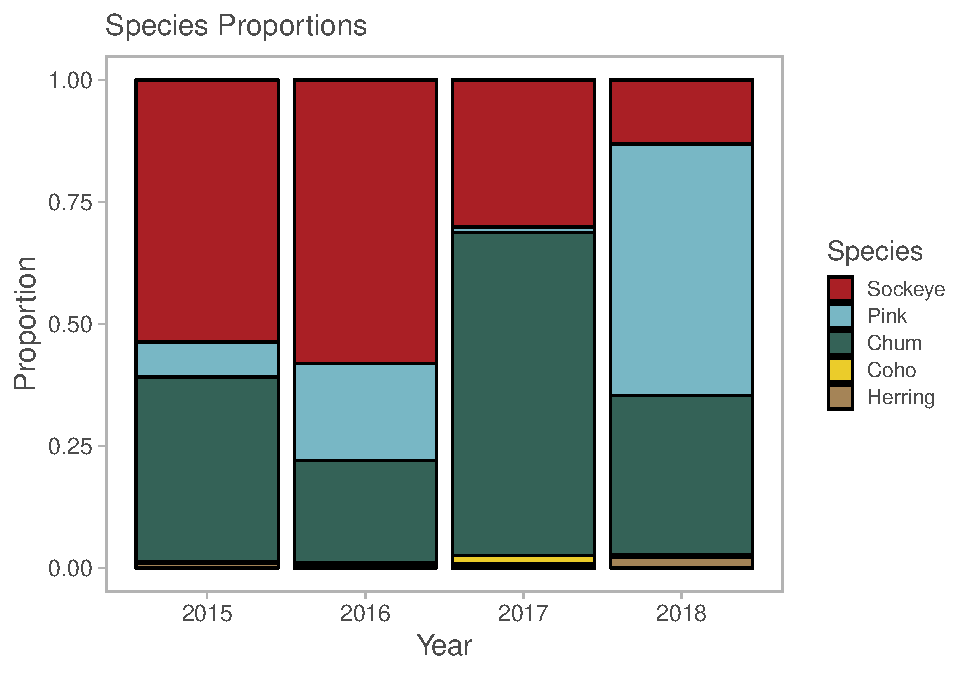
\includegraphics[width=0.9\linewidth]{Migration_Observations_Report_files/figure-latex/proportion-plot-1} \caption{The annual proportion of fish captured in the Discovery Islands and Johnstone Strait combined.}\label{fig:proportion-plot}
\end{figure}

\begin{figure}[H]
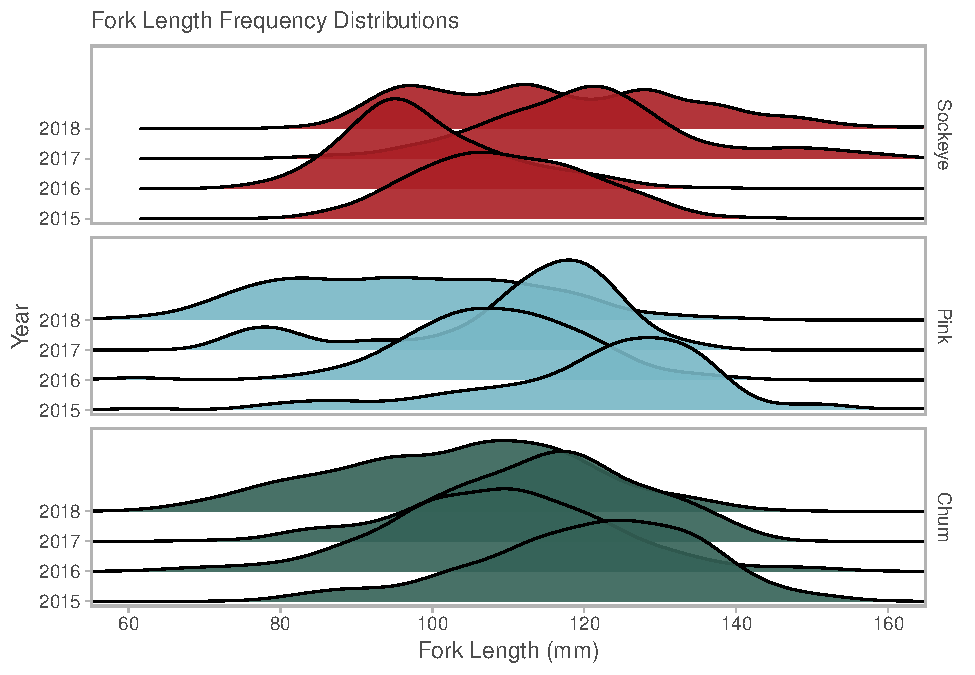
\includegraphics[width=0.9\linewidth]{Migration_Observations_Report_files/figure-latex/length-plot-1} \caption{Distributions of juvenile salmon fork lengths for each year in the Discovery Islands and Johnstone Strait. Note that these distributions contain multiple age classes.}\label{fig:length-plot}
\end{figure}

\begin{figure}[H]
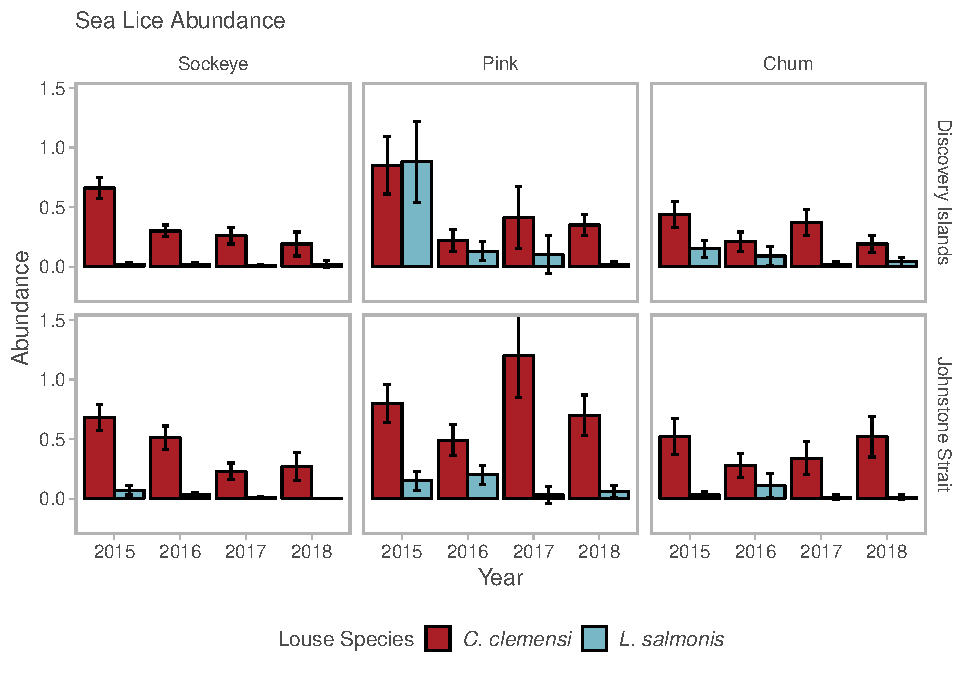
\includegraphics[width=0.9\linewidth]{Migration_Observations_Report_files/figure-latex/sealice-abundance-plot-1} \caption{The abundance of motile sea lice on juvenile salmon in the Discovery Islands and Johnstone Strait. The numbers under each bar indicate the sample size and the error bars indicate the 95 percent confidence region.}\label{fig:sealice-abundance-plot}
\end{figure}

\begin{figure}[H]
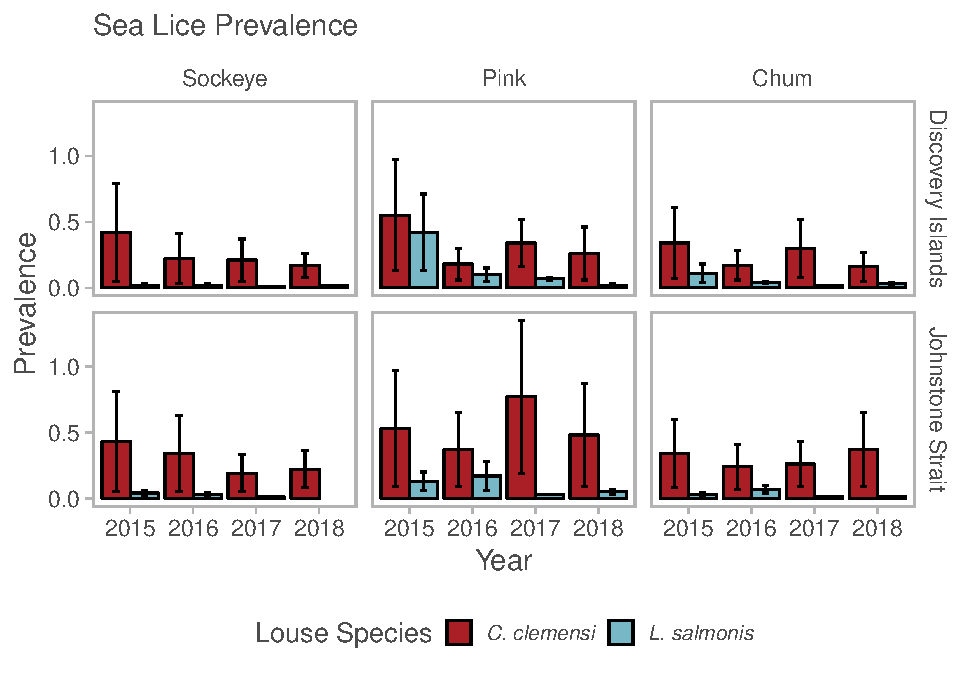
\includegraphics[width=0.9\linewidth]{Migration_Observations_Report_files/figure-latex/sealice-prevalence-plot-1} \caption{The prevalence of motile sea lice on juvenile salmon in the Discovery Islands and Johnstone Strait. The numbers under each bar indicate the sample size and the error bars indicate the 95 percent confidence region.}\label{fig:sealice-prevalence-plot}
\end{figure}

\begin{figure}[H]
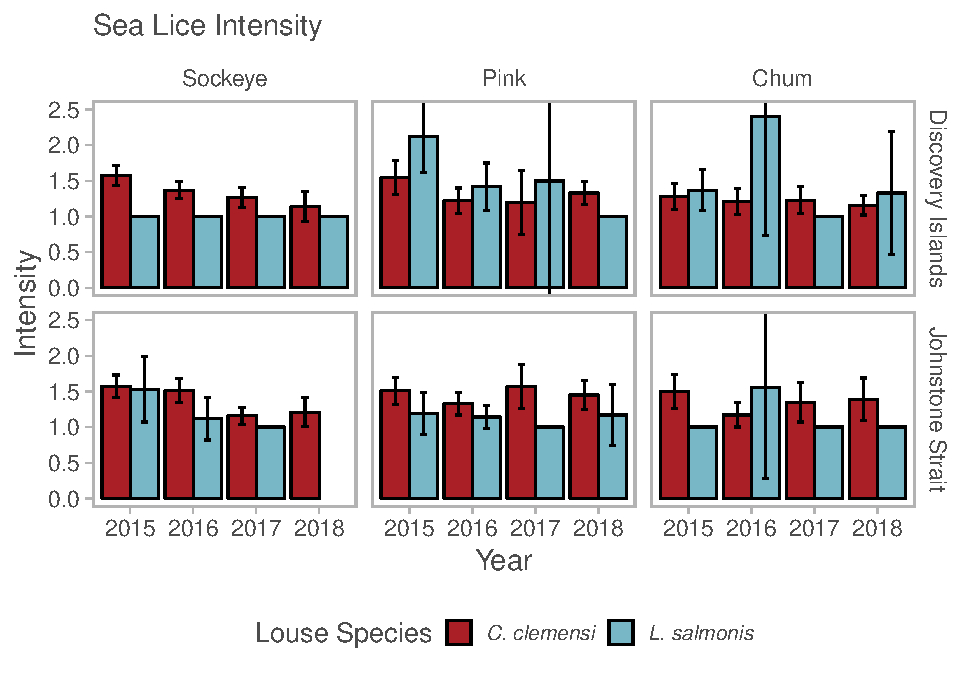
\includegraphics[width=0.9\linewidth]{Migration_Observations_Report_files/figure-latex/sealice-intensity-plot-1} \caption{The intensity of motile sea lice (average number of lice when > 1 louse is present) on juvenile salmon in the Discovery Islands and Johnstone Strait. The numbers under each bar indicate the sample size and the error bars indicate the 95 percent confidence region.}\label{fig:sealice-intensity-plot}
\end{figure}

\begin{figure}[H]
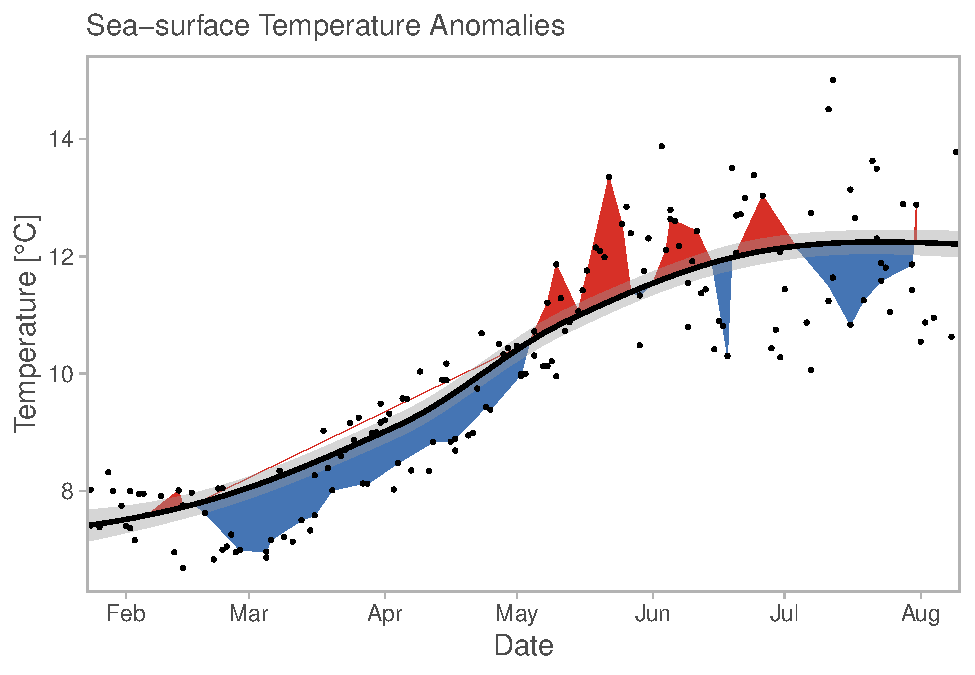
\includegraphics[width=0.9\linewidth]{Migration_Observations_Report_files/figure-latex/sst-plot-1} \caption{Sea-surace temperature (top 30 m) at station QU39 in the northern Strait of Georgia is the solid black line which is a LOESS regression based on temperatures from 2015-2018 representing the time series average. Blue areas represent temperatures from 2018 that are below average, red areas represent above average temperatures. The shaded grey area is 1 SE of the LOESS regression. The black dots are the daily minimum and maximum temperatures observed over the time series.}\label{fig:sst-plot}
\end{figure}

\hypertarget{tables}{%
\section{Tables}\label{tables}}

\begin{longtable}[]{@{}rllrr@{}}
\caption{\label{tab:z-scores-table} Key salmon health, growth, and migration annual estimates. Migration timing estimates are the median capture date in the Discovery Islands, catch intensity estimates are the mean catch when greater than one sockeye are caught in the Discovery Islands and Johnstone Strait combined, length estimates are the mean fork length (mm) in both regions combined, parasite loads are mean abundance for motile lice from both regions combined, and SST is the mean sea-surface temperature in degrees celcius at station QU39 in the northern Strait of Georgia. Standard deviation is denoted by SD and is the within-year standard deviation (note no SD for median capture dates). Z score is the number of standard deviations the annual estimate is away from the time series mean.}\tabularnewline
\toprule
Year & Parameter & Estimate & SD & Z score\tabularnewline
\midrule
\endfirsthead
\toprule
Year & Parameter & Estimate & SD & Z score\tabularnewline
\midrule
\endhead
2015 & Sockeye Migration Timing & May 23 & NA & -0.71\tabularnewline
2016 & Sockeye Migration Timing & May 28 & NA & 0.00\tabularnewline
2017 & Sockeye Migration Timing & June 07 & NA & 1.41\tabularnewline
2018 & Sockeye Migration Timing & May 23 & NA & -0.71\tabularnewline
2015 & Sockeye Catch Intensity & 272.2 & 479.80 & 0.68\tabularnewline
2016 & Sockeye Catch Intensity & 307.2 & 431.70 & 1.03\tabularnewline
2017 & Sockeye Catch Intensity & 131.5 & 158.20 & -0.76\tabularnewline
2018 & Sockeye Catch Intensity & 113.7 & 289.90 & -0.95\tabularnewline
2015 & Sockeye Length & 109.7 & 11.14 & -0.20\tabularnewline
2016 & Sockeye Length & 99.1 & 10.66 & -1.32\tabularnewline
2017 & Sockeye Length & 120.4 & 14.03 & 0.94\tabularnewline
2018 & Sockeye Length & 116.9 & 18.54 & 0.58\tabularnewline
2015 & Sockeye Parasite Loads & 0.71 & 0.04 & 1.40\tabularnewline
2016 & Sockeye Parasite Loads & 0.425 & 0.16 & 0.04\tabularnewline
2017 & Sockeye Parasite Loads & 0.255 & 0.04 & -0.65\tabularnewline
2018 & Sockeye Parasite Loads & 0.24 & 0.04 & -0.79\tabularnewline
2015 & Pink Migration Timing & July 07 & NA & 1.43\tabularnewline
2016 & Pink Migration Timing & June 15 & NA & -0.16\tabularnewline
2017 & Pink Migration Timing & June 05 & NA & -0.89\tabularnewline
2018 & Pink Migration Timing & June 12 & NA & -0.38\tabularnewline
2015 & Pink Catch Intensity & 65.3 & 145.80 & -0.48\tabularnewline
2016 & Pink Catch Intensity & 109.9 & 169.10 & -0.26\tabularnewline
2017 & Pink Catch Intensity & 11.3 & 15.90 & -0.73\tabularnewline
2018 & Pink Catch Intensity & 475.1 & 802.90 & 1.47\tabularnewline
2015 & Pink Length & 121.4 & 16.25 & 1.20\tabularnewline
2016 & Pink Length & 108.2 & 11.92 & -0.09\tabularnewline
2017 & Pink Length & 110.6 & 15.19 & 0.14\tabularnewline
2018 & Pink Length & 96.4 & 16.56 & -1.24\tabularnewline
2015 & Pink Parasite Loads & 1.335 & 0.56 & 1.16\tabularnewline
2016 & Pink Parasite Loads & 0.52 & 0.23 & -0.91\tabularnewline
2017 & Pink Parasite Loads & 0.875 & 0.50 & 0.50\tabularnewline
2018 & Pink Parasite Loads & 0.565 & 0.28 & -0.76\tabularnewline
2015 & Chum Migration Timing & June 05 & NA & -1.09\tabularnewline
2016 & Chum Migration Timing & June 15 & NA & 0.06\tabularnewline
2017 & Chum Migration Timing & June 26 & NA & 1.32\tabularnewline
2018 & Chum Migration Timing & June 12 & NA & -0.29\tabularnewline
2015 & Chum Catch Intensity & 194.6 & 283.40 & -0.37\tabularnewline
2016 & Chum Catch Intensity & 113.4 & 175.10 & -1.24\tabularnewline
2017 & Chum Catch Intensity & 298.6 & 378.60 & 0.74\tabularnewline
2018 & Chum Catch Intensity & 310.8 & 518.50 & 0.87\tabularnewline
2015 & Chum Length & 120.7 & 14.29 & 1.19\tabularnewline
2016 & Chum Length & 108.6 & 14.38 & -0.44\tabularnewline
2017 & Chum Length & 114.5 & 13.47 & 0.36\tabularnewline
2018 & Chum Length & 103.5 & 16.03 & -1.12\tabularnewline
2015 & Chum Parasite Loads & 0.565 & 0.02 & 1.48\tabularnewline
2016 & Chum Parasite Loads & 0.34 & 0.07 & -0.72\tabularnewline
2017 & Chum Parasite Loads & 0.37 & 0.01 & -0.43\tabularnewline
2018 & Chum Parasite Loads & 0.38 & 0.21 & -0.33\tabularnewline
2015 & SST & 11.55 & 1.18 & -0.04\tabularnewline
2016 & SST & 11.56 & 0.95 & 0.02\tabularnewline
2017 & SST & 11.28 & 1.14 & -1.21\tabularnewline
2018 & SST & 11.84 & 1.02 & 1.23\tabularnewline
\bottomrule
\end{longtable}

\begin{longtable}[]{@{}llllllr@{}}
\caption{\label{tab:migration-timing-table} Migration timing statistics for the cumulative catch of sockeye, pink, and chum salmon in the Discovery Islands in 2018, compared to the time-series average (2015 - 2018). Q1 is when 25 \% of the species passed through the regions, peak date is the median when 50 \% passed through, Q3 is 75\%, and Spread is the difference between Peak Date and Q1. The region DI indicates the Discovery Islands while for species SO is sockeye, PI is pink, and CU is chum.}\tabularnewline
\toprule
Year & Region & Species & Q1 & Peak Date & Q3 & Spread\tabularnewline
\midrule
\endfirsthead
\toprule
Year & Region & Species & Q1 & Peak Date & Q3 & Spread\tabularnewline
\midrule
\endhead
2015 - 2018 & DI & CU & June 06 & June 15 & June 23 & 8\tabularnewline
2015 - 2018 & DI & PI & June 05 & June 13 & June 13 & 9\tabularnewline
2015 - 2018 & DI & SO & May 26 & May 28 & June 04 & 2\tabularnewline
2015 - 2018 & JS & CU & June 11 & June 19 & June 23 & 7\tabularnewline
2015 - 2018 & JS & PI & June 16 & June 23 & June 23 & 6\tabularnewline
2015 - 2018 & JS & SO & June 03 & June 05 & June 18 & 3\tabularnewline
2015 & DI & CU & June 03 & June 05 & June 22 & 2\tabularnewline
2015 & DI & SO & May 23 & May 23 & June 01 & 0\tabularnewline
2015 & JS & CU & June 09 & June 16 & June 19 & 7\tabularnewline
2015 & JS & SO & May 26 & May 29 & June 13 & 3\tabularnewline
2016 & DI & CU & June 02 & June 15 & June 15 & 13\tabularnewline
2016 & DI & PI & June 02 & June 15 & June 15 & 13\tabularnewline
2016 & DI & SO & May 24 & May 28 & June 04 & 4\tabularnewline
2016 & JS & CU & June 02 & June 10 & June 24 & 8\tabularnewline
2016 & JS & PI & June 18 & June 24 & June 24 & 6\tabularnewline
2016 & JS & SO & June 02 & June 03 & June 18 & 1\tabularnewline
2017 & DI & CU & June 13 & June 26 & July 04 & 13\tabularnewline
2017 & DI & SO & June 05 & June 07 & June 07 & 2\tabularnewline
2017 & JS & CU & June 20 & June 27 & June 28 & 7\tabularnewline
2017 & JS & SO & June 06 & June 14 & June 21 & 8\tabularnewline
2018 & DI & CU & June 07 & June 12 & June 20 & 5\tabularnewline
2018 & DI & PI & June 07 & June 12 & June 12 & 5\tabularnewline
2018 & DI & SO & May 23 & May 23 & June 04 & 0\tabularnewline
2018 & JS & CU & June 14 & June 21 & June 23 & 7\tabularnewline
2018 & JS & PI & June 14 & June 21 & June 23 & 7\tabularnewline
2018 & JS & SO & June 07 & June 07 & June 21 & 0\tabularnewline
\bottomrule
\end{longtable}

\begin{longtable}[]{@{}rlr@{}}
\caption{\label{tab:catch-intensity-table} Catch intensity---our proxy for abundance---for sockeye, pink, and chum in the Discovery Islands and Johnstone Strait combined.}\tabularnewline
\toprule
Year & Species & Catch Intensity\tabularnewline
\midrule
\endfirsthead
\toprule
Year & Species & Catch Intensity\tabularnewline
\midrule
\endhead
2015 & Chum & 194.6\tabularnewline
2015 & Pink & 65.3\tabularnewline
2015 & Sockeye & 272.2\tabularnewline
2016 & Chum & 113.4\tabularnewline
2016 & Pink & 109.9\tabularnewline
2016 & Sockeye & 307.2\tabularnewline
2017 & Chum & 298.6\tabularnewline
2017 & Pink & 11.3\tabularnewline
2017 & Sockeye & 131.5\tabularnewline
2018 & Chum & 310.8\tabularnewline
2018 & Pink & 475.1\tabularnewline
2018 & Sockeye & 113.7\tabularnewline
\bottomrule
\end{longtable}

\begin{longtable}[]{@{}lllrrr@{}}
\caption{\label{tab:length-table} Mean fork lengths for each year, species, and region with the 95 \% confidence interval (95\% CI). The column n indicates the number of fish measured.}\tabularnewline
\toprule
Year & Region & Species & N & Fork Length & CI\tabularnewline
\midrule
\endfirsthead
\toprule
Year & Region & Species & N & Fork Length & CI\tabularnewline
\midrule
\endhead
2015 & DI & SO & 455 & 108.9 & 1.0\tabularnewline
2015 & DI & PI & 47 & 109.6 & 5.5\tabularnewline
2015 & DI & CU & 121 & 115.5 & 2.8\tabularnewline
2015 & JS & SO & 334 & 110.7 & 1.2\tabularnewline
2015 & JS & PI & 98 & 127.1 & 2.2\tabularnewline
2015 & JS & CU & 112 & 126.4 & 2.0\tabularnewline
2016 & DI & SO & 516 & 97.6 & 0.9\tabularnewline
2016 & DI & PI & 96 & 103.9 & 2.6\tabularnewline
2016 & DI & CU & 124 & 103.3 & 2.6\tabularnewline
2016 & JS & SO & 316 & 101.5 & 1.1\tabularnewline
2016 & JS & PI & 94 & 112.6 & 1.9\tabularnewline
2016 & JS & CU & 104 & 115.0 & 2.1\tabularnewline
2017 & DI & SO & 260 & 121.3 & 2.0\tabularnewline
2017 & DI & PI & 17 & 90.9 & 8.6\tabularnewline
2017 & DI & CU & 111 & 106.2 & 2.4\tabularnewline
2017 & JS & SO & 220 & 119.4 & 1.4\tabularnewline
2017 & JS & PI & 51 & 117.1 & 1.9\tabularnewline
2017 & JS & CU & 151 & 120.7 & 1.6\tabularnewline
2018 & DI & SO & 84 & 116.2 & 3.6\tabularnewline
2018 & DI & PI & 205 & 87.8 & 1.8\tabularnewline
2018 & DI & CU & 190 & 97.4 & 2.3\tabularnewline
2018 & JS & SO & 85 & 117.6 & 4.4\tabularnewline
2018 & JS & PI & 110 & 112.4 & 1.8\tabularnewline
2018 & JS & CU & 110 & 114.2 & 1.8\tabularnewline
\bottomrule
\end{longtable}

\begin{longtable}[]{@{}rrrrrr@{}}
\caption{\label{tab:proportion-table} The species proportions of total catch in each year for sockeye, pink, chum, herring, coho, and Chinook.}\tabularnewline
\toprule
Year & Chum & Coho & Herring & Pink & Sockeye\tabularnewline
\midrule
\endfirsthead
\toprule
Year & Chum & Coho & Herring & Pink & Sockeye\tabularnewline
\midrule
\endhead
2015 & 0.378 & 0.003 & 0.009 & 0.072 & 0.537\tabularnewline
2016 & 0.210 & 0.006 & 0.005 & 0.200 & 0.580\tabularnewline
2017 & 0.661 & 0.018 & 0.008 & 0.012 & 0.301\tabularnewline
2018 & 0.326 & 0.006 & 0.022 & 0.515 & 0.131\tabularnewline
\bottomrule
\end{longtable}

\begin{longtable}[]{@{}llllrlll@{}}
\caption{\label{tab:sealice-table} Mean sea-louse abundance, prevalence, and intensity (as defined in Margolis et al.~1990) across the time series (2015-2018) for each fish, region, and year. 95\% confidence intervals were calculated from annual averages. The region DI indicates the Discovery Islands and JS Johnstone Strait.}\tabularnewline
\toprule
\begin{minipage}[b]{0.04\columnwidth}\raggedright
Year\strut
\end{minipage} & \begin{minipage}[b]{0.06\columnwidth}\raggedright
Region\strut
\end{minipage} & \begin{minipage}[b]{0.07\columnwidth}\raggedright
Species\strut
\end{minipage} & \begin{minipage}[b]{0.13\columnwidth}\raggedright
Louse Species\strut
\end{minipage} & \begin{minipage}[b]{0.03\columnwidth}\raggedleft
n\strut
\end{minipage} & \begin{minipage}[b]{0.15\columnwidth}\raggedright
Abundance, 95\% CI\strut
\end{minipage} & \begin{minipage}[b]{0.16\columnwidth}\raggedright
Prevalence, 95\% CI\strut
\end{minipage} & \begin{minipage}[b]{0.15\columnwidth}\raggedright
Intensity, 95\% CI\strut
\end{minipage}\tabularnewline
\midrule
\endfirsthead
\toprule
\begin{minipage}[b]{0.04\columnwidth}\raggedright
Year\strut
\end{minipage} & \begin{minipage}[b]{0.06\columnwidth}\raggedright
Region\strut
\end{minipage} & \begin{minipage}[b]{0.07\columnwidth}\raggedright
Species\strut
\end{minipage} & \begin{minipage}[b]{0.13\columnwidth}\raggedright
Louse Species\strut
\end{minipage} & \begin{minipage}[b]{0.03\columnwidth}\raggedleft
n\strut
\end{minipage} & \begin{minipage}[b]{0.15\columnwidth}\raggedright
Abundance, 95\% CI\strut
\end{minipage} & \begin{minipage}[b]{0.16\columnwidth}\raggedright
Prevalence, 95\% CI\strut
\end{minipage} & \begin{minipage}[b]{0.15\columnwidth}\raggedright
Intensity, 95\% CI\strut
\end{minipage}\tabularnewline
\midrule
\endhead
\begin{minipage}[t]{0.04\columnwidth}\raggedright
2015\strut
\end{minipage} & \begin{minipage}[t]{0.06\columnwidth}\raggedright
DI\strut
\end{minipage} & \begin{minipage}[t]{0.07\columnwidth}\raggedright
Chum\strut
\end{minipage} & \begin{minipage}[t]{0.13\columnwidth}\raggedright
Motile Caligus\strut
\end{minipage} & \begin{minipage}[t]{0.03\columnwidth}\raggedleft
179\strut
\end{minipage} & \begin{minipage}[t]{0.15\columnwidth}\raggedright
0.44 +/- 0.11\strut
\end{minipage} & \begin{minipage}[t]{0.16\columnwidth}\raggedright
0.34 +/- 0.27\strut
\end{minipage} & \begin{minipage}[t]{0.15\columnwidth}\raggedright
1.28 +/- 0.18\strut
\end{minipage}\tabularnewline
\begin{minipage}[t]{0.04\columnwidth}\raggedright
2015\strut
\end{minipage} & \begin{minipage}[t]{0.06\columnwidth}\raggedright
DI\strut
\end{minipage} & \begin{minipage}[t]{0.07\columnwidth}\raggedright
Pink\strut
\end{minipage} & \begin{minipage}[t]{0.13\columnwidth}\raggedright
Motile Caligus\strut
\end{minipage} & \begin{minipage}[t]{0.03\columnwidth}\raggedleft
60\strut
\end{minipage} & \begin{minipage}[t]{0.15\columnwidth}\raggedright
0.85 +/- 0.24\strut
\end{minipage} & \begin{minipage}[t]{0.16\columnwidth}\raggedright
0.55 +/- 0.42\strut
\end{minipage} & \begin{minipage}[t]{0.15\columnwidth}\raggedright
1.55 +/- 0.24\strut
\end{minipage}\tabularnewline
\begin{minipage}[t]{0.04\columnwidth}\raggedright
2015\strut
\end{minipage} & \begin{minipage}[t]{0.06\columnwidth}\raggedright
DI\strut
\end{minipage} & \begin{minipage}[t]{0.07\columnwidth}\raggedright
Sockeye\strut
\end{minipage} & \begin{minipage}[t]{0.13\columnwidth}\raggedright
Motile Caligus\strut
\end{minipage} & \begin{minipage}[t]{0.03\columnwidth}\raggedleft
425\strut
\end{minipage} & \begin{minipage}[t]{0.15\columnwidth}\raggedright
0.66 +/- 0.09\strut
\end{minipage} & \begin{minipage}[t]{0.16\columnwidth}\raggedright
0.42 +/- 0.37\strut
\end{minipage} & \begin{minipage}[t]{0.15\columnwidth}\raggedright
1.58 +/- 0.14\strut
\end{minipage}\tabularnewline
\begin{minipage}[t]{0.04\columnwidth}\raggedright
2015\strut
\end{minipage} & \begin{minipage}[t]{0.06\columnwidth}\raggedright
DI\strut
\end{minipage} & \begin{minipage}[t]{0.07\columnwidth}\raggedright
Chum\strut
\end{minipage} & \begin{minipage}[t]{0.13\columnwidth}\raggedright
Motile Lep\strut
\end{minipage} & \begin{minipage}[t]{0.03\columnwidth}\raggedleft
179\strut
\end{minipage} & \begin{minipage}[t]{0.15\columnwidth}\raggedright
0.15 +/- 0.07\strut
\end{minipage} & \begin{minipage}[t]{0.16\columnwidth}\raggedright
0.11 +/- 0.07\strut
\end{minipage} & \begin{minipage}[t]{0.15\columnwidth}\raggedright
1.37 +/- 0.29\strut
\end{minipage}\tabularnewline
\begin{minipage}[t]{0.04\columnwidth}\raggedright
2015\strut
\end{minipage} & \begin{minipage}[t]{0.06\columnwidth}\raggedright
DI\strut
\end{minipage} & \begin{minipage}[t]{0.07\columnwidth}\raggedright
Pink\strut
\end{minipage} & \begin{minipage}[t]{0.13\columnwidth}\raggedright
Motile Lep\strut
\end{minipage} & \begin{minipage}[t]{0.03\columnwidth}\raggedleft
60\strut
\end{minipage} & \begin{minipage}[t]{0.15\columnwidth}\raggedright
0.88 +/- 0.34\strut
\end{minipage} & \begin{minipage}[t]{0.16\columnwidth}\raggedright
0.42 +/- 0.29\strut
\end{minipage} & \begin{minipage}[t]{0.15\columnwidth}\raggedright
2.12 +/- 0.5\strut
\end{minipage}\tabularnewline
\begin{minipage}[t]{0.04\columnwidth}\raggedright
2015\strut
\end{minipage} & \begin{minipage}[t]{0.06\columnwidth}\raggedright
DI\strut
\end{minipage} & \begin{minipage}[t]{0.07\columnwidth}\raggedright
Sockeye\strut
\end{minipage} & \begin{minipage}[t]{0.13\columnwidth}\raggedright
Motile Lep\strut
\end{minipage} & \begin{minipage}[t]{0.03\columnwidth}\raggedleft
425\strut
\end{minipage} & \begin{minipage}[t]{0.15\columnwidth}\raggedright
0.02 +/- 0.01\strut
\end{minipage} & \begin{minipage}[t]{0.16\columnwidth}\raggedright
0.02 +/- 0.01\strut
\end{minipage} & \begin{minipage}[t]{0.15\columnwidth}\raggedright
1 +/- 0\strut
\end{minipage}\tabularnewline
\begin{minipage}[t]{0.04\columnwidth}\raggedright
2015\strut
\end{minipage} & \begin{minipage}[t]{0.06\columnwidth}\raggedright
JS\strut
\end{minipage} & \begin{minipage}[t]{0.07\columnwidth}\raggedright
Chum\strut
\end{minipage} & \begin{minipage}[t]{0.13\columnwidth}\raggedright
Motile Caligus\strut
\end{minipage} & \begin{minipage}[t]{0.03\columnwidth}\raggedleft
122\strut
\end{minipage} & \begin{minipage}[t]{0.15\columnwidth}\raggedright
0.52 +/- 0.15\strut
\end{minipage} & \begin{minipage}[t]{0.16\columnwidth}\raggedright
0.34 +/- 0.26\strut
\end{minipage} & \begin{minipage}[t]{0.15\columnwidth}\raggedright
1.5 +/- 0.24\strut
\end{minipage}\tabularnewline
\begin{minipage}[t]{0.04\columnwidth}\raggedright
2015\strut
\end{minipage} & \begin{minipage}[t]{0.06\columnwidth}\raggedright
JS\strut
\end{minipage} & \begin{minipage}[t]{0.07\columnwidth}\raggedright
Pink\strut
\end{minipage} & \begin{minipage}[t]{0.13\columnwidth}\raggedright
Motile Caligus\strut
\end{minipage} & \begin{minipage}[t]{0.03\columnwidth}\raggedleft
127\strut
\end{minipage} & \begin{minipage}[t]{0.15\columnwidth}\raggedright
0.8 +/- 0.16\strut
\end{minipage} & \begin{minipage}[t]{0.16\columnwidth}\raggedright
0.53 +/- 0.44\strut
\end{minipage} & \begin{minipage}[t]{0.15\columnwidth}\raggedright
1.51 +/- 0.19\strut
\end{minipage}\tabularnewline
\begin{minipage}[t]{0.04\columnwidth}\raggedright
2015\strut
\end{minipage} & \begin{minipage}[t]{0.06\columnwidth}\raggedright
JS\strut
\end{minipage} & \begin{minipage}[t]{0.07\columnwidth}\raggedright
Sockeye\strut
\end{minipage} & \begin{minipage}[t]{0.13\columnwidth}\raggedright
Motile Caligus\strut
\end{minipage} & \begin{minipage}[t]{0.03\columnwidth}\raggedleft
348\strut
\end{minipage} & \begin{minipage}[t]{0.15\columnwidth}\raggedright
0.68 +/- 0.11\strut
\end{minipage} & \begin{minipage}[t]{0.16\columnwidth}\raggedright
0.43 +/- 0.38\strut
\end{minipage} & \begin{minipage}[t]{0.15\columnwidth}\raggedright
1.57 +/- 0.16\strut
\end{minipage}\tabularnewline
\begin{minipage}[t]{0.04\columnwidth}\raggedright
2015\strut
\end{minipage} & \begin{minipage}[t]{0.06\columnwidth}\raggedright
JS\strut
\end{minipage} & \begin{minipage}[t]{0.07\columnwidth}\raggedright
Chum\strut
\end{minipage} & \begin{minipage}[t]{0.13\columnwidth}\raggedright
Motile Lep\strut
\end{minipage} & \begin{minipage}[t]{0.03\columnwidth}\raggedleft
122\strut
\end{minipage} & \begin{minipage}[t]{0.15\columnwidth}\raggedright
0.03 +/- 0.03\strut
\end{minipage} & \begin{minipage}[t]{0.16\columnwidth}\raggedright
0.03 +/- 0.01\strut
\end{minipage} & \begin{minipage}[t]{0.15\columnwidth}\raggedright
1 +/- 0\strut
\end{minipage}\tabularnewline
\begin{minipage}[t]{0.04\columnwidth}\raggedright
2015\strut
\end{minipage} & \begin{minipage}[t]{0.06\columnwidth}\raggedright
JS\strut
\end{minipage} & \begin{minipage}[t]{0.07\columnwidth}\raggedright
Pink\strut
\end{minipage} & \begin{minipage}[t]{0.13\columnwidth}\raggedright
Motile Lep\strut
\end{minipage} & \begin{minipage}[t]{0.03\columnwidth}\raggedleft
127\strut
\end{minipage} & \begin{minipage}[t]{0.15\columnwidth}\raggedright
0.15 +/- 0.08\strut
\end{minipage} & \begin{minipage}[t]{0.16\columnwidth}\raggedright
0.13 +/- 0.07\strut
\end{minipage} & \begin{minipage}[t]{0.15\columnwidth}\raggedright
1.19 +/- 0.29\strut
\end{minipage}\tabularnewline
\begin{minipage}[t]{0.04\columnwidth}\raggedright
2015\strut
\end{minipage} & \begin{minipage}[t]{0.06\columnwidth}\raggedright
JS\strut
\end{minipage} & \begin{minipage}[t]{0.07\columnwidth}\raggedright
Sockeye\strut
\end{minipage} & \begin{minipage}[t]{0.13\columnwidth}\raggedright
Motile Lep\strut
\end{minipage} & \begin{minipage}[t]{0.03\columnwidth}\raggedleft
348\strut
\end{minipage} & \begin{minipage}[t]{0.15\columnwidth}\raggedright
0.07 +/- 0.04\strut
\end{minipage} & \begin{minipage}[t]{0.16\columnwidth}\raggedright
0.04 +/- 0.02\strut
\end{minipage} & \begin{minipage}[t]{0.15\columnwidth}\raggedright
1.53 +/- 0.46\strut
\end{minipage}\tabularnewline
\begin{minipage}[t]{0.04\columnwidth}\raggedright
2016\strut
\end{minipage} & \begin{minipage}[t]{0.06\columnwidth}\raggedright
DI\strut
\end{minipage} & \begin{minipage}[t]{0.07\columnwidth}\raggedright
Chum\strut
\end{minipage} & \begin{minipage}[t]{0.13\columnwidth}\raggedright
Motile Caligus\strut
\end{minipage} & \begin{minipage}[t]{0.03\columnwidth}\raggedleft
139\strut
\end{minipage} & \begin{minipage}[t]{0.15\columnwidth}\raggedright
0.21 +/- 0.08\strut
\end{minipage} & \begin{minipage}[t]{0.16\columnwidth}\raggedright
0.17 +/- 0.11\strut
\end{minipage} & \begin{minipage}[t]{0.15\columnwidth}\raggedright
1.21 +/- 0.18\strut
\end{minipage}\tabularnewline
\begin{minipage}[t]{0.04\columnwidth}\raggedright
2016\strut
\end{minipage} & \begin{minipage}[t]{0.06\columnwidth}\raggedright
DI\strut
\end{minipage} & \begin{minipage}[t]{0.07\columnwidth}\raggedright
Pink\strut
\end{minipage} & \begin{minipage}[t]{0.13\columnwidth}\raggedright
Motile Caligus\strut
\end{minipage} & \begin{minipage}[t]{0.03\columnwidth}\raggedleft
126\strut
\end{minipage} & \begin{minipage}[t]{0.15\columnwidth}\raggedright
0.22 +/- 0.09\strut
\end{minipage} & \begin{minipage}[t]{0.16\columnwidth}\raggedright
0.18 +/- 0.12\strut
\end{minipage} & \begin{minipage}[t]{0.15\columnwidth}\raggedright
1.22 +/- 0.18\strut
\end{minipage}\tabularnewline
\begin{minipage}[t]{0.04\columnwidth}\raggedright
2016\strut
\end{minipage} & \begin{minipage}[t]{0.06\columnwidth}\raggedright
DI\strut
\end{minipage} & \begin{minipage}[t]{0.07\columnwidth}\raggedright
Sockeye\strut
\end{minipage} & \begin{minipage}[t]{0.13\columnwidth}\raggedright
Motile Caligus\strut
\end{minipage} & \begin{minipage}[t]{0.03\columnwidth}\raggedleft
611\strut
\end{minipage} & \begin{minipage}[t]{0.15\columnwidth}\raggedright
0.3 +/- 0.05\strut
\end{minipage} & \begin{minipage}[t]{0.16\columnwidth}\raggedright
0.22 +/- 0.19\strut
\end{minipage} & \begin{minipage}[t]{0.15\columnwidth}\raggedright
1.37 +/- 0.12\strut
\end{minipage}\tabularnewline
\begin{minipage}[t]{0.04\columnwidth}\raggedright
2016\strut
\end{minipage} & \begin{minipage}[t]{0.06\columnwidth}\raggedright
DI\strut
\end{minipage} & \begin{minipage}[t]{0.07\columnwidth}\raggedright
Chum\strut
\end{minipage} & \begin{minipage}[t]{0.13\columnwidth}\raggedright
Motile Lep\strut
\end{minipage} & \begin{minipage}[t]{0.03\columnwidth}\raggedleft
139\strut
\end{minipage} & \begin{minipage}[t]{0.15\columnwidth}\raggedright
0.09 +/- 0.08\strut
\end{minipage} & \begin{minipage}[t]{0.16\columnwidth}\raggedright
0.04 +/- 0.01\strut
\end{minipage} & \begin{minipage}[t]{0.15\columnwidth}\raggedright
2.4 +/- 1.67\strut
\end{minipage}\tabularnewline
\begin{minipage}[t]{0.04\columnwidth}\raggedright
2016\strut
\end{minipage} & \begin{minipage}[t]{0.06\columnwidth}\raggedright
DI\strut
\end{minipage} & \begin{minipage}[t]{0.07\columnwidth}\raggedright
Pink\strut
\end{minipage} & \begin{minipage}[t]{0.13\columnwidth}\raggedright
Motile Lep\strut
\end{minipage} & \begin{minipage}[t]{0.03\columnwidth}\raggedleft
126\strut
\end{minipage} & \begin{minipage}[t]{0.15\columnwidth}\raggedright
0.13 +/- 0.08\strut
\end{minipage} & \begin{minipage}[t]{0.16\columnwidth}\raggedright
0.1 +/- 0.05\strut
\end{minipage} & \begin{minipage}[t]{0.15\columnwidth}\raggedright
1.42 +/- 0.33\strut
\end{minipage}\tabularnewline
\begin{minipage}[t]{0.04\columnwidth}\raggedright
2016\strut
\end{minipage} & \begin{minipage}[t]{0.06\columnwidth}\raggedright
DI\strut
\end{minipage} & \begin{minipage}[t]{0.07\columnwidth}\raggedright
Sockeye\strut
\end{minipage} & \begin{minipage}[t]{0.13\columnwidth}\raggedright
Motile Lep\strut
\end{minipage} & \begin{minipage}[t]{0.03\columnwidth}\raggedleft
611\strut
\end{minipage} & \begin{minipage}[t]{0.15\columnwidth}\raggedright
0.02 +/- 0.01\strut
\end{minipage} & \begin{minipage}[t]{0.16\columnwidth}\raggedright
0.02 +/- 0.01\strut
\end{minipage} & \begin{minipage}[t]{0.15\columnwidth}\raggedright
1 +/- 0\strut
\end{minipage}\tabularnewline
\begin{minipage}[t]{0.04\columnwidth}\raggedright
2016\strut
\end{minipage} & \begin{minipage}[t]{0.06\columnwidth}\raggedright
JS\strut
\end{minipage} & \begin{minipage}[t]{0.07\columnwidth}\raggedright
Chum\strut
\end{minipage} & \begin{minipage}[t]{0.13\columnwidth}\raggedright
Motile Caligus\strut
\end{minipage} & \begin{minipage}[t]{0.03\columnwidth}\raggedleft
127\strut
\end{minipage} & \begin{minipage}[t]{0.15\columnwidth}\raggedright
0.28 +/- 0.1\strut
\end{minipage} & \begin{minipage}[t]{0.16\columnwidth}\raggedright
0.24 +/- 0.17\strut
\end{minipage} & \begin{minipage}[t]{0.15\columnwidth}\raggedright
1.17 +/- 0.17\strut
\end{minipage}\tabularnewline
\begin{minipage}[t]{0.04\columnwidth}\raggedright
2016\strut
\end{minipage} & \begin{minipage}[t]{0.06\columnwidth}\raggedright
JS\strut
\end{minipage} & \begin{minipage}[t]{0.07\columnwidth}\raggedright
Pink\strut
\end{minipage} & \begin{minipage}[t]{0.13\columnwidth}\raggedright
Motile Caligus\strut
\end{minipage} & \begin{minipage}[t]{0.03\columnwidth}\raggedleft
123\strut
\end{minipage} & \begin{minipage}[t]{0.15\columnwidth}\raggedright
0.49 +/- 0.13\strut
\end{minipage} & \begin{minipage}[t]{0.16\columnwidth}\raggedright
0.37 +/- 0.28\strut
\end{minipage} & \begin{minipage}[t]{0.15\columnwidth}\raggedright
1.33 +/- 0.16\strut
\end{minipage}\tabularnewline
\begin{minipage}[t]{0.04\columnwidth}\raggedright
2016\strut
\end{minipage} & \begin{minipage}[t]{0.06\columnwidth}\raggedright
JS\strut
\end{minipage} & \begin{minipage}[t]{0.07\columnwidth}\raggedright
Sockeye\strut
\end{minipage} & \begin{minipage}[t]{0.13\columnwidth}\raggedright
Motile Caligus\strut
\end{minipage} & \begin{minipage}[t]{0.03\columnwidth}\raggedleft
311\strut
\end{minipage} & \begin{minipage}[t]{0.15\columnwidth}\raggedright
0.51 +/- 0.1\strut
\end{minipage} & \begin{minipage}[t]{0.16\columnwidth}\raggedright
0.34 +/- 0.29\strut
\end{minipage} & \begin{minipage}[t]{0.15\columnwidth}\raggedright
1.51 +/- 0.17\strut
\end{minipage}\tabularnewline
\begin{minipage}[t]{0.04\columnwidth}\raggedright
2016\strut
\end{minipage} & \begin{minipage}[t]{0.06\columnwidth}\raggedright
JS\strut
\end{minipage} & \begin{minipage}[t]{0.07\columnwidth}\raggedright
Chum\strut
\end{minipage} & \begin{minipage}[t]{0.13\columnwidth}\raggedright
Motile Lep\strut
\end{minipage} & \begin{minipage}[t]{0.03\columnwidth}\raggedleft
127\strut
\end{minipage} & \begin{minipage}[t]{0.15\columnwidth}\raggedright
0.11 +/- 0.1\strut
\end{minipage} & \begin{minipage}[t]{0.16\columnwidth}\raggedright
0.07 +/- 0.03\strut
\end{minipage} & \begin{minipage}[t]{0.15\columnwidth}\raggedright
1.56 +/- 1.28\strut
\end{minipage}\tabularnewline
\begin{minipage}[t]{0.04\columnwidth}\raggedright
2016\strut
\end{minipage} & \begin{minipage}[t]{0.06\columnwidth}\raggedright
JS\strut
\end{minipage} & \begin{minipage}[t]{0.07\columnwidth}\raggedright
Pink\strut
\end{minipage} & \begin{minipage}[t]{0.13\columnwidth}\raggedright
Motile Lep\strut
\end{minipage} & \begin{minipage}[t]{0.03\columnwidth}\raggedleft
123\strut
\end{minipage} & \begin{minipage}[t]{0.15\columnwidth}\raggedright
0.2 +/- 0.08\strut
\end{minipage} & \begin{minipage}[t]{0.16\columnwidth}\raggedright
0.17 +/- 0.11\strut
\end{minipage} & \begin{minipage}[t]{0.15\columnwidth}\raggedright
1.14 +/- 0.16\strut
\end{minipage}\tabularnewline
\begin{minipage}[t]{0.04\columnwidth}\raggedright
2016\strut
\end{minipage} & \begin{minipage}[t]{0.06\columnwidth}\raggedright
JS\strut
\end{minipage} & \begin{minipage}[t]{0.07\columnwidth}\raggedright
Sockeye\strut
\end{minipage} & \begin{minipage}[t]{0.13\columnwidth}\raggedright
Motile Lep\strut
\end{minipage} & \begin{minipage}[t]{0.03\columnwidth}\raggedleft
311\strut
\end{minipage} & \begin{minipage}[t]{0.15\columnwidth}\raggedright
0.03 +/- 0.02\strut
\end{minipage} & \begin{minipage}[t]{0.16\columnwidth}\raggedright
0.03 +/- 0.01\strut
\end{minipage} & \begin{minipage}[t]{0.15\columnwidth}\raggedright
1.12 +/- 0.3\strut
\end{minipage}\tabularnewline
\begin{minipage}[t]{0.04\columnwidth}\raggedright
2017\strut
\end{minipage} & \begin{minipage}[t]{0.06\columnwidth}\raggedright
DI\strut
\end{minipage} & \begin{minipage}[t]{0.07\columnwidth}\raggedright
Chum\strut
\end{minipage} & \begin{minipage}[t]{0.13\columnwidth}\raggedright
Motile Caligus\strut
\end{minipage} & \begin{minipage}[t]{0.03\columnwidth}\raggedleft
130\strut
\end{minipage} & \begin{minipage}[t]{0.15\columnwidth}\raggedright
0.37 +/- 0.11\strut
\end{minipage} & \begin{minipage}[t]{0.16\columnwidth}\raggedright
0.3 +/- 0.22\strut
\end{minipage} & \begin{minipage}[t]{0.15\columnwidth}\raggedright
1.23 +/- 0.19\strut
\end{minipage}\tabularnewline
\begin{minipage}[t]{0.04\columnwidth}\raggedright
2017\strut
\end{minipage} & \begin{minipage}[t]{0.06\columnwidth}\raggedright
DI\strut
\end{minipage} & \begin{minipage}[t]{0.07\columnwidth}\raggedright
Pink\strut
\end{minipage} & \begin{minipage}[t]{0.13\columnwidth}\raggedright
Motile Caligus\strut
\end{minipage} & \begin{minipage}[t]{0.03\columnwidth}\raggedleft
29\strut
\end{minipage} & \begin{minipage}[t]{0.15\columnwidth}\raggedright
0.41 +/- 0.26\strut
\end{minipage} & \begin{minipage}[t]{0.16\columnwidth}\raggedright
0.34 +/- 0.18\strut
\end{minipage} & \begin{minipage}[t]{0.15\columnwidth}\raggedright
1.2 +/- 0.45\strut
\end{minipage}\tabularnewline
\begin{minipage}[t]{0.04\columnwidth}\raggedright
2017\strut
\end{minipage} & \begin{minipage}[t]{0.06\columnwidth}\raggedright
DI\strut
\end{minipage} & \begin{minipage}[t]{0.07\columnwidth}\raggedright
Sockeye\strut
\end{minipage} & \begin{minipage}[t]{0.13\columnwidth}\raggedright
Motile Caligus\strut
\end{minipage} & \begin{minipage}[t]{0.03\columnwidth}\raggedleft
271\strut
\end{minipage} & \begin{minipage}[t]{0.15\columnwidth}\raggedright
0.26 +/- 0.07\strut
\end{minipage} & \begin{minipage}[t]{0.16\columnwidth}\raggedright
0.21 +/- 0.16\strut
\end{minipage} & \begin{minipage}[t]{0.15\columnwidth}\raggedright
1.27 +/- 0.14\strut
\end{minipage}\tabularnewline
\begin{minipage}[t]{0.04\columnwidth}\raggedright
2017\strut
\end{minipage} & \begin{minipage}[t]{0.06\columnwidth}\raggedright
DI\strut
\end{minipage} & \begin{minipage}[t]{0.07\columnwidth}\raggedright
Chum\strut
\end{minipage} & \begin{minipage}[t]{0.13\columnwidth}\raggedright
Motile Lep\strut
\end{minipage} & \begin{minipage}[t]{0.03\columnwidth}\raggedleft
130\strut
\end{minipage} & \begin{minipage}[t]{0.15\columnwidth}\raggedright
0.02 +/- 0.02\strut
\end{minipage} & \begin{minipage}[t]{0.16\columnwidth}\raggedright
0.02 +/- 0\strut
\end{minipage} & \begin{minipage}[t]{0.15\columnwidth}\raggedright
1 +/- 0\strut
\end{minipage}\tabularnewline
\begin{minipage}[t]{0.04\columnwidth}\raggedright
2017\strut
\end{minipage} & \begin{minipage}[t]{0.06\columnwidth}\raggedright
DI\strut
\end{minipage} & \begin{minipage}[t]{0.07\columnwidth}\raggedright
Pink\strut
\end{minipage} & \begin{minipage}[t]{0.13\columnwidth}\raggedright
Motile Lep\strut
\end{minipage} & \begin{minipage}[t]{0.03\columnwidth}\raggedleft
29\strut
\end{minipage} & \begin{minipage}[t]{0.15\columnwidth}\raggedright
0.1 +/- 0.16\strut
\end{minipage} & \begin{minipage}[t]{0.16\columnwidth}\raggedright
0.07 +/- 0.01\strut
\end{minipage} & \begin{minipage}[t]{0.15\columnwidth}\raggedright
1.5 +/- 6.35\strut
\end{minipage}\tabularnewline
\begin{minipage}[t]{0.04\columnwidth}\raggedright
2017\strut
\end{minipage} & \begin{minipage}[t]{0.06\columnwidth}\raggedright
DI\strut
\end{minipage} & \begin{minipage}[t]{0.07\columnwidth}\raggedright
Sockeye\strut
\end{minipage} & \begin{minipage}[t]{0.13\columnwidth}\raggedright
Motile Lep\strut
\end{minipage} & \begin{minipage}[t]{0.03\columnwidth}\raggedleft
271\strut
\end{minipage} & \begin{minipage}[t]{0.15\columnwidth}\raggedright
0.01 +/- 0.01\strut
\end{minipage} & \begin{minipage}[t]{0.16\columnwidth}\raggedright
0.01 +/- 0\strut
\end{minipage} & \begin{minipage}[t]{0.15\columnwidth}\raggedright
1 +/- 0\strut
\end{minipage}\tabularnewline
\begin{minipage}[t]{0.04\columnwidth}\raggedright
2017\strut
\end{minipage} & \begin{minipage}[t]{0.06\columnwidth}\raggedright
JS\strut
\end{minipage} & \begin{minipage}[t]{0.07\columnwidth}\raggedright
Chum\strut
\end{minipage} & \begin{minipage}[t]{0.13\columnwidth}\raggedright
Motile Caligus\strut
\end{minipage} & \begin{minipage}[t]{0.03\columnwidth}\raggedleft
90\strut
\end{minipage} & \begin{minipage}[t]{0.15\columnwidth}\raggedright
0.34 +/- 0.14\strut
\end{minipage} & \begin{minipage}[t]{0.16\columnwidth}\raggedright
0.26 +/- 0.17\strut
\end{minipage} & \begin{minipage}[t]{0.15\columnwidth}\raggedright
1.35 +/- 0.28\strut
\end{minipage}\tabularnewline
\begin{minipage}[t]{0.04\columnwidth}\raggedright
2017\strut
\end{minipage} & \begin{minipage}[t]{0.06\columnwidth}\raggedright
JS\strut
\end{minipage} & \begin{minipage}[t]{0.07\columnwidth}\raggedright
Pink\strut
\end{minipage} & \begin{minipage}[t]{0.13\columnwidth}\raggedright
Motile Caligus\strut
\end{minipage} & \begin{minipage}[t]{0.03\columnwidth}\raggedleft
30\strut
\end{minipage} & \begin{minipage}[t]{0.15\columnwidth}\raggedright
1.2 +/- 0.35\strut
\end{minipage} & \begin{minipage}[t]{0.16\columnwidth}\raggedright
0.77 +/- 0.58\strut
\end{minipage} & \begin{minipage}[t]{0.15\columnwidth}\raggedright
1.57 +/- 0.31\strut
\end{minipage}\tabularnewline
\begin{minipage}[t]{0.04\columnwidth}\raggedright
2017\strut
\end{minipage} & \begin{minipage}[t]{0.06\columnwidth}\raggedright
JS\strut
\end{minipage} & \begin{minipage}[t]{0.07\columnwidth}\raggedright
Sockeye\strut
\end{minipage} & \begin{minipage}[t]{0.13\columnwidth}\raggedright
Motile Caligus\strut
\end{minipage} & \begin{minipage}[t]{0.03\columnwidth}\raggedleft
191\strut
\end{minipage} & \begin{minipage}[t]{0.15\columnwidth}\raggedright
0.23 +/- 0.07\strut
\end{minipage} & \begin{minipage}[t]{0.16\columnwidth}\raggedright
0.19 +/- 0.14\strut
\end{minipage} & \begin{minipage}[t]{0.15\columnwidth}\raggedright
1.16 +/- 0.12\strut
\end{minipage}\tabularnewline
\begin{minipage}[t]{0.04\columnwidth}\raggedright
2017\strut
\end{minipage} & \begin{minipage}[t]{0.06\columnwidth}\raggedright
JS\strut
\end{minipage} & \begin{minipage}[t]{0.07\columnwidth}\raggedright
Chum\strut
\end{minipage} & \begin{minipage}[t]{0.13\columnwidth}\raggedright
Motile Lep\strut
\end{minipage} & \begin{minipage}[t]{0.03\columnwidth}\raggedleft
90\strut
\end{minipage} & \begin{minipage}[t]{0.15\columnwidth}\raggedright
0.01 +/- 0.02\strut
\end{minipage} & \begin{minipage}[t]{0.16\columnwidth}\raggedright
0.01 +/- 0\strut
\end{minipage} & \begin{minipage}[t]{0.15\columnwidth}\raggedright
1 +/- NA\strut
\end{minipage}\tabularnewline
\begin{minipage}[t]{0.04\columnwidth}\raggedright
2017\strut
\end{minipage} & \begin{minipage}[t]{0.06\columnwidth}\raggedright
JS\strut
\end{minipage} & \begin{minipage}[t]{0.07\columnwidth}\raggedright
Pink\strut
\end{minipage} & \begin{minipage}[t]{0.13\columnwidth}\raggedright
Motile Lep\strut
\end{minipage} & \begin{minipage}[t]{0.03\columnwidth}\raggedleft
30\strut
\end{minipage} & \begin{minipage}[t]{0.15\columnwidth}\raggedright
0.03 +/- 0.07\strut
\end{minipage} & \begin{minipage}[t]{0.16\columnwidth}\raggedright
0.03 +/- 0\strut
\end{minipage} & \begin{minipage}[t]{0.15\columnwidth}\raggedright
1 +/- NA\strut
\end{minipage}\tabularnewline
\begin{minipage}[t]{0.04\columnwidth}\raggedright
2017\strut
\end{minipage} & \begin{minipage}[t]{0.06\columnwidth}\raggedright
JS\strut
\end{minipage} & \begin{minipage}[t]{0.07\columnwidth}\raggedright
Sockeye\strut
\end{minipage} & \begin{minipage}[t]{0.13\columnwidth}\raggedright
Motile Lep\strut
\end{minipage} & \begin{minipage}[t]{0.03\columnwidth}\raggedleft
191\strut
\end{minipage} & \begin{minipage}[t]{0.15\columnwidth}\raggedright
0.01 +/- 0.01\strut
\end{minipage} & \begin{minipage}[t]{0.16\columnwidth}\raggedright
0.01 +/- 0\strut
\end{minipage} & \begin{minipage}[t]{0.15\columnwidth}\raggedright
1 +/- NA\strut
\end{minipage}\tabularnewline
\begin{minipage}[t]{0.04\columnwidth}\raggedright
2018\strut
\end{minipage} & \begin{minipage}[t]{0.06\columnwidth}\raggedright
DI\strut
\end{minipage} & \begin{minipage}[t]{0.07\columnwidth}\raggedright
Chum\strut
\end{minipage} & \begin{minipage}[t]{0.13\columnwidth}\raggedright
Motile Caligus\strut
\end{minipage} & \begin{minipage}[t]{0.03\columnwidth}\raggedleft
190\strut
\end{minipage} & \begin{minipage}[t]{0.15\columnwidth}\raggedright
0.19 +/- 0.07\strut
\end{minipage} & \begin{minipage}[t]{0.16\columnwidth}\raggedright
0.16 +/- 0.11\strut
\end{minipage} & \begin{minipage}[t]{0.15\columnwidth}\raggedright
1.16 +/- 0.14\strut
\end{minipage}\tabularnewline
\begin{minipage}[t]{0.04\columnwidth}\raggedright
2018\strut
\end{minipage} & \begin{minipage}[t]{0.06\columnwidth}\raggedright
DI\strut
\end{minipage} & \begin{minipage}[t]{0.07\columnwidth}\raggedright
Pink\strut
\end{minipage} & \begin{minipage}[t]{0.13\columnwidth}\raggedright
Motile Caligus\strut
\end{minipage} & \begin{minipage}[t]{0.03\columnwidth}\raggedleft
205\strut
\end{minipage} & \begin{minipage}[t]{0.15\columnwidth}\raggedright
0.35 +/- 0.09\strut
\end{minipage} & \begin{minipage}[t]{0.16\columnwidth}\raggedright
0.26 +/- 0.2\strut
\end{minipage} & \begin{minipage}[t]{0.15\columnwidth}\raggedright
1.33 +/- 0.16\strut
\end{minipage}\tabularnewline
\begin{minipage}[t]{0.04\columnwidth}\raggedright
2018\strut
\end{minipage} & \begin{minipage}[t]{0.06\columnwidth}\raggedright
DI\strut
\end{minipage} & \begin{minipage}[t]{0.07\columnwidth}\raggedright
Sockeye\strut
\end{minipage} & \begin{minipage}[t]{0.13\columnwidth}\raggedright
Motile Caligus\strut
\end{minipage} & \begin{minipage}[t]{0.03\columnwidth}\raggedleft
84\strut
\end{minipage} & \begin{minipage}[t]{0.15\columnwidth}\raggedright
0.19 +/- 0.1\strut
\end{minipage} & \begin{minipage}[t]{0.16\columnwidth}\raggedright
0.17 +/- 0.09\strut
\end{minipage} & \begin{minipage}[t]{0.15\columnwidth}\raggedright
1.14 +/- 0.21\strut
\end{minipage}\tabularnewline
\begin{minipage}[t]{0.04\columnwidth}\raggedright
2018\strut
\end{minipage} & \begin{minipage}[t]{0.06\columnwidth}\raggedright
DI\strut
\end{minipage} & \begin{minipage}[t]{0.07\columnwidth}\raggedright
Chum\strut
\end{minipage} & \begin{minipage}[t]{0.13\columnwidth}\raggedright
Motile Lep\strut
\end{minipage} & \begin{minipage}[t]{0.03\columnwidth}\raggedleft
190\strut
\end{minipage} & \begin{minipage}[t]{0.15\columnwidth}\raggedright
0.04 +/- 0.04\strut
\end{minipage} & \begin{minipage}[t]{0.16\columnwidth}\raggedright
0.03 +/- 0.01\strut
\end{minipage} & \begin{minipage}[t]{0.15\columnwidth}\raggedright
1.33 +/- 0.86\strut
\end{minipage}\tabularnewline
\begin{minipage}[t]{0.04\columnwidth}\raggedright
2018\strut
\end{minipage} & \begin{minipage}[t]{0.06\columnwidth}\raggedright
DI\strut
\end{minipage} & \begin{minipage}[t]{0.07\columnwidth}\raggedright
Pink\strut
\end{minipage} & \begin{minipage}[t]{0.13\columnwidth}\raggedright
Motile Lep\strut
\end{minipage} & \begin{minipage}[t]{0.03\columnwidth}\raggedleft
205\strut
\end{minipage} & \begin{minipage}[t]{0.15\columnwidth}\raggedright
0.02 +/- 0.02\strut
\end{minipage} & \begin{minipage}[t]{0.16\columnwidth}\raggedright
0.02 +/- 0.01\strut
\end{minipage} & \begin{minipage}[t]{0.15\columnwidth}\raggedright
1 +/- 0\strut
\end{minipage}\tabularnewline
\begin{minipage}[t]{0.04\columnwidth}\raggedright
2018\strut
\end{minipage} & \begin{minipage}[t]{0.06\columnwidth}\raggedright
DI\strut
\end{minipage} & \begin{minipage}[t]{0.07\columnwidth}\raggedright
Sockeye\strut
\end{minipage} & \begin{minipage}[t]{0.13\columnwidth}\raggedright
Motile Lep\strut
\end{minipage} & \begin{minipage}[t]{0.03\columnwidth}\raggedleft
84\strut
\end{minipage} & \begin{minipage}[t]{0.15\columnwidth}\raggedright
0.02 +/- 0.03\strut
\end{minipage} & \begin{minipage}[t]{0.16\columnwidth}\raggedright
0.02 +/- 0\strut
\end{minipage} & \begin{minipage}[t]{0.15\columnwidth}\raggedright
1 +/- 0\strut
\end{minipage}\tabularnewline
\begin{minipage}[t]{0.04\columnwidth}\raggedright
2018\strut
\end{minipage} & \begin{minipage}[t]{0.06\columnwidth}\raggedright
JS\strut
\end{minipage} & \begin{minipage}[t]{0.07\columnwidth}\raggedright
Chum\strut
\end{minipage} & \begin{minipage}[t]{0.13\columnwidth}\raggedright
Motile Caligus\strut
\end{minipage} & \begin{minipage}[t]{0.03\columnwidth}\raggedleft
110\strut
\end{minipage} & \begin{minipage}[t]{0.15\columnwidth}\raggedright
0.52 +/- 0.17\strut
\end{minipage} & \begin{minipage}[t]{0.16\columnwidth}\raggedright
0.37 +/- 0.28\strut
\end{minipage} & \begin{minipage}[t]{0.15\columnwidth}\raggedright
1.39 +/- 0.3\strut
\end{minipage}\tabularnewline
\begin{minipage}[t]{0.04\columnwidth}\raggedright
2018\strut
\end{minipage} & \begin{minipage}[t]{0.06\columnwidth}\raggedright
JS\strut
\end{minipage} & \begin{minipage}[t]{0.07\columnwidth}\raggedright
Pink\strut
\end{minipage} & \begin{minipage}[t]{0.13\columnwidth}\raggedright
Motile Caligus\strut
\end{minipage} & \begin{minipage}[t]{0.03\columnwidth}\raggedleft
110\strut
\end{minipage} & \begin{minipage}[t]{0.15\columnwidth}\raggedright
0.7 +/- 0.17\strut
\end{minipage} & \begin{minipage}[t]{0.16\columnwidth}\raggedright
0.48 +/- 0.39\strut
\end{minipage} & \begin{minipage}[t]{0.15\columnwidth}\raggedright
1.45 +/- 0.2\strut
\end{minipage}\tabularnewline
\begin{minipage}[t]{0.04\columnwidth}\raggedright
2018\strut
\end{minipage} & \begin{minipage}[t]{0.06\columnwidth}\raggedright
JS\strut
\end{minipage} & \begin{minipage}[t]{0.07\columnwidth}\raggedright
Sockeye\strut
\end{minipage} & \begin{minipage}[t]{0.13\columnwidth}\raggedright
Motile Caligus\strut
\end{minipage} & \begin{minipage}[t]{0.03\columnwidth}\raggedleft
85\strut
\end{minipage} & \begin{minipage}[t]{0.15\columnwidth}\raggedright
0.27 +/- 0.12\strut
\end{minipage} & \begin{minipage}[t]{0.16\columnwidth}\raggedright
0.22 +/- 0.14\strut
\end{minipage} & \begin{minipage}[t]{0.15\columnwidth}\raggedright
1.21 +/- 0.2\strut
\end{minipage}\tabularnewline
\begin{minipage}[t]{0.04\columnwidth}\raggedright
2018\strut
\end{minipage} & \begin{minipage}[t]{0.06\columnwidth}\raggedright
JS\strut
\end{minipage} & \begin{minipage}[t]{0.07\columnwidth}\raggedright
Chum\strut
\end{minipage} & \begin{minipage}[t]{0.13\columnwidth}\raggedright
Motile Lep\strut
\end{minipage} & \begin{minipage}[t]{0.03\columnwidth}\raggedleft
110\strut
\end{minipage} & \begin{minipage}[t]{0.15\columnwidth}\raggedright
0.01 +/- 0.02\strut
\end{minipage} & \begin{minipage}[t]{0.16\columnwidth}\raggedright
0.01 +/- 0\strut
\end{minipage} & \begin{minipage}[t]{0.15\columnwidth}\raggedright
1 +/- NA\strut
\end{minipage}\tabularnewline
\begin{minipage}[t]{0.04\columnwidth}\raggedright
2018\strut
\end{minipage} & \begin{minipage}[t]{0.06\columnwidth}\raggedright
JS\strut
\end{minipage} & \begin{minipage}[t]{0.07\columnwidth}\raggedright
Pink\strut
\end{minipage} & \begin{minipage}[t]{0.13\columnwidth}\raggedright
Motile Lep\strut
\end{minipage} & \begin{minipage}[t]{0.03\columnwidth}\raggedleft
110\strut
\end{minipage} & \begin{minipage}[t]{0.15\columnwidth}\raggedright
0.06 +/- 0.05\strut
\end{minipage} & \begin{minipage}[t]{0.16\columnwidth}\raggedright
0.05 +/- 0.02\strut
\end{minipage} & \begin{minipage}[t]{0.15\columnwidth}\raggedright
1.17 +/- 0.43\strut
\end{minipage}\tabularnewline
\begin{minipage}[t]{0.04\columnwidth}\raggedright
2018\strut
\end{minipage} & \begin{minipage}[t]{0.06\columnwidth}\raggedright
JS\strut
\end{minipage} & \begin{minipage}[t]{0.07\columnwidth}\raggedright
Sockeye\strut
\end{minipage} & \begin{minipage}[t]{0.13\columnwidth}\raggedright
Motile Lep\strut
\end{minipage} & \begin{minipage}[t]{0.03\columnwidth}\raggedleft
85\strut
\end{minipage} & \begin{minipage}[t]{0.15\columnwidth}\raggedright
0 +/- 0\strut
\end{minipage} & \begin{minipage}[t]{0.16\columnwidth}\raggedright
NA +/- NA\strut
\end{minipage} & \begin{minipage}[t]{0.15\columnwidth}\raggedright
NA +/- NA\strut
\end{minipage}\tabularnewline
\bottomrule
\end{longtable}

\hypertarget{references}{%
\section*{References}\label{references}}
\addcontentsline{toc}{section}{References}

\hypertarget{refs}{}
\leavevmode\hypertarget{ref-Beamish2001}{}%
Beamish, R., and C. Mahnken. 2001. ``A critical size and period hypothesis to explain natural regulation of salmon abundance and the linkage to climate and climate change.'' \emph{Progress in Oceanography} 49: 423--37.

\leavevmode\hypertarget{ref-Beamish2012}{}%
Beamish, R., C. Neville, R. Sweeting, and K. Lange. 2012. ``The synchronous failure of juvenile pacific salmon and herring production in the strait of georgia in 2007 and the poor return of sockeye salmon to the Fraser river in 2009.'' \emph{Marine and Coastal Fisheries} 4 (1): 403--14. \url{https://doi.org/10.1080/19425120.2012.676607}.

\leavevmode\hypertarget{ref-Chandler2017}{}%
Chandler, P.C., S.A. King, and J. Boldt. 2017. ``State of the Physical , Biological and Selected Fishery Resources of Pacific Canadian Marine Ecosystems in 2016 Can. Tech. Rep. Fish. Aquat. Sci.'' 3225 (243). Sidney, BC: Fisheries; Oceans Canada.

\leavevmode\hypertarget{ref-Godwin2015}{}%
Godwin, Sean C, Lawrence M Dill, John D Reynolds, and Martin Krkosek. 2015. ``Sea Lice, sockeye salmon, and foraging competition: lousy fish are lousy competitors.'' \emph{Canadian Journal of Fisheries and Aquatic Sciences} 1120 (March): 778--82. \url{https://doi.org/10.1139/cjfas-2014-0284}.

\leavevmode\hypertarget{ref-Heard1991}{}%
Heard, William R. 1991. ``Life History of Pink Salmon.'' In \emph{Pacific Salmon Life Histories}, edited by C. Groot and L. Margolis, 121. 2029 West Mall, Vancouver, BC V6T 1Z2: UBC Press.

\leavevmode\hypertarget{ref-Hunt2018}{}%
Hunt, Brian P.V., Brett T. Johnson, Sean C. Godwin, Martin Krkošek, Evgeny A Pakhomov, and Luke A Rogers. 2018. ``The Hakai Institute Juvenile Salmon Program : Early Life History Drivers of Marine Survival in Sockeye , Pink and Chum Salmon in British Columbia.'' Institute for the Oceans; Fisheries; Department of Earth, Ocean; Atmospheric Sciences, University of British Columbia, Hakai Institute, Earth to Ocean Research Group, Simon Fraser University, Department of Ecology; Evolutionary Biology, Univer.

\leavevmode\hypertarget{ref-Margolis1990}{}%
Margolis, L., G. W. Esch, A.M. Kuris, and G.A. Schad. 1990. ``The Use of Ecological Terms in Parasitology (Report of an Ad Hoc Committee of the American Society of Parasitologists).'' \emph{The Journal of Parisitology} 68 (1): 131--33. \url{https://doi.org/10.2307/3281335}.

\leavevmode\hypertarget{ref-Neville2016}{}%
Neville, Chrys-Ellen, Stewart Johnson, Terry Beacham, Timber Whitehouse, Joe Tadey, and Marc Trudel. 2016. ``Initial Estimates from an Integrated Study Examining the Residence Period and Migration Timing of Juvenile Sockeye Salmon from the Fraser River through Coastal Waters of British Columbia.'' \emph{North Pacific Anadromous Fish Commission Bulletin} 6 (1): 45--60. \url{https://doi.org/10.23849/npafcb6/45.60}.

\leavevmode\hypertarget{ref-Patanasatienkul2013}{}%
Patanasatienkul, Thitiwan, Javier Sanchez, Erin E. Rees, Martin Krkošek, Simon R.M. Jones, and Crawford W. Revie. 2013. ``Sea lice infestations on juvenile chum and pink salmon in the Broughton Archipelago, Canada, from 2003 to 2012.'' \emph{Diseases of Aquatic Organisms} 105 (2): 149--61. \url{https://doi.org/10.3354/dao02616}.

\leavevmode\hypertarget{ref-Peterman2010}{}%
Peterman, Randall M, D Marmorek, B Beckman, M Bradford, M Lapointe, N Mantua, Brian Riddell, et al. 2010. ``Synthesis of evidence from a workshop on the decline of Fraser River sockeye. June 15-17, 2010. A Report to the Pacific Salmon Commission.'' August. Vancovuer, British Columbia: Pacific Salmon Commission.

\leavevmode\hypertarget{ref-R}{}%
R Core Team. 2017. \emph{R: A Language and Environment for Statistical Computing}. Vienna, Austria: R Foundation for Statistical Computing. \url{https://www.R-project.org/}.



\end{document}
